\section{Answer Set Programming for explainable planning}
\subsection{Planning problem definition in FOL}
\begin{minipage}[t]{0.2\textwidth}
    \begin{figure}[H]
        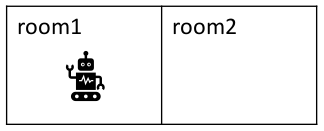
\includegraphics[width=0.9\textwidth]{img/env.png}
        \centering
    \end{figure}
\end{minipage}
\begin{minipage}[t]{0.8\textwidth}
    Given the problem on the left where a robot starting in room A has to change room.\\
    We define the knowledge base in FOL:
    \setstretch{0.5}
    \begin{itemize}
        \item Rooms A, B with possible constant values room1, room2
        \item Location (state) $at(A)$
        \item Action predicate $move(A, B)$
        \begin{itemize}
            \item Precondition: $move(A, B) \leftarrow at(A)$
            \item Effect 1 (post-cond.): $at(B) \leftarrow move(A, B)$
            \item Effect 2: $not\;at(A) \leftarrow move(A, B)$
            \item Constraint: $move(A, B),\;A \ne B$
        \end{itemize}
        \item Initial state: $at(room1)$
        \item Goal state: $at(room2)$
    \end{itemize}
\end{minipage}
\singlespacing
\subsubsection*{Model Checking}
To solve the problem with Model Checking we have to first enumetare all possibilites.\\
What's the plan?
\begin{itemize}
    \item Start from the initial state $at(room1)$
    \item Which variables can we substitute (ground) in $move(A, B)$?
    \begin{itemize}
        \item $move(room1, room2)$
        \item $move(room2, room1)$
        \item $move(room1, room1)$
        \item $move(room2, room2)$
    \end{itemize}
\end{itemize}

\vspace*{1pt}
Now knowing that we are $at(room1)$ we can use our \textbf{precondition} to remove actions that violates those.\\

\begin{minipage}[t]{0.5\textwidth}
    \setstretch{0.5}
    \begin{itemize}
        \item Rooms A, B with possible constant values room1, room2
        \item Location (state) $at(A)$
        \item Action predicate $move(A, B)$
        \begin{itemize}
            \item \textcolor{red}{Precondition: $move(A, B) \leftarrow at(A)$}
            \item Effect 1 (post-cond.): $at(B) \leftarrow move(A, B)$
            \item Effect 2: $not\;at(A) \leftarrow move(A, B)$
            \item Constraint: $move(A, B),\;A \ne B$
        \end{itemize}
        \item Initial state: $at(room1)$
        \item Goal state: $at(room2)$
    \end{itemize}
\end{minipage}
\begin{minipage}[t]{0.8\textwidth}
    \begin{itemize}
        \item Start from the initial state $at(room1)$
        \item Which variables can we substitute (ground) in $move(A, B)$?
        \begin{itemize}
            \item $move(room1, room2)$
            \item \textcolor{red}{\st{$move(room2, room1)$}}
            \item $move(room1, room1)$
            \item \textcolor{red}{\st{$move(room2, room2)$}}
        \end{itemize}
    \end{itemize}
\end{minipage}
\newpage
\noindent
Now knowing that we are $at(room1)$ we can use our constraint to remove actions that violates that.\\

\begin{minipage}[t]{0.5\textwidth}
    \setstretch{0.5}
    \begin{itemize}
        \item Rooms A, B with possible constant values room1, room2
        \item Location (state) $at(A)$
        \item Action predicate $move(A, B)$
        \begin{itemize}
            \item \textcolor{red}{Precondition: $move(A, B) \leftarrow at(A)$}
            \item Effect 1 (post-cond.): $at(B) \leftarrow move(A, B)$
            \item Effect 2: $not\;at(A) \leftarrow move(A, B)$
            \item \textcolor{blue}{Constraint: $move(A, B),\;A \ne B$}
        \end{itemize}
        \item Initial state: $at(room1)$
        \item Goal state: $at(room2)$
    \end{itemize}
\end{minipage}
\begin{minipage}[t]{0.8\textwidth}
    \begin{itemize}
        \item Start from the initial state $at(room1)$
        \item Which variables can we substitute (ground) in $move(A, B)$?
        \begin{itemize}
            \item $\bm{move(room1, room2)}$
            \item \textcolor{red}{\st{$move(room2, room1)$}}
            \item \textcolor{blue}{\st{$move(room1, room1)$}}
            \item \textcolor{red}{\st{$move(room2, room2)$}}
        \end{itemize}
    \end{itemize}
\end{minipage}

\vspace{0.5cm}
Now by applying preconditions and constraints we found that the only feasible action is $move(room1, room2)$.
Progating that action we can see that we reach the goal.

\begin{minipage}[t]{0.5\textwidth}
    \setstretch{0.5}
    \begin{itemize}
        \item Rooms A, B with possible constant values room1, room2
        \item Location (state) $at(A)$
        \item Action predicate $move(A, B)$
        \begin{itemize}
            \item \textcolor{red}{Precondition: $move(A, B) \leftarrow at(A)$}
            \item \textcolor{ForestGreen}{Effect 1 (post-cond.): $at(B) \leftarrow move(A, B)$}
            \item Effect 2: $not\;at(A) \leftarrow move(A, B)$
            \item \textcolor{blue}{Constraint: $move(A, B),\;A \ne B$}
        \end{itemize}
        \item Initial state: $at(room1)$
        \item Goal state: $at(room2)$
    \end{itemize}
\end{minipage}
\begin{minipage}[t]{0.8\textwidth}
    \begin{itemize}
        \item Start from the initial state $at(room1)$
        \item Which variables can we substitute (ground) in $move(A, B)$?
        \begin{itemize}
            \item $\bm{move(room1, room2)}$
            \item \textcolor{red}{\st{$move(room2, room1)$}}
            \item \textcolor{blue}{\st{$move(room1, room1)$}}
            \item \textcolor{red}{\st{$move(room2, room2)$}}
        \end{itemize}
    \end{itemize}
\end{minipage}
\vspace{0.1cm}

Which term may I infer? \textcolor{ForestGreen}{$at(room2)$}. This means that we reached the goal and so
$\{move(room1,room2)\}$ is a solution for this planning problem.

\subsubsection*{Absurd Reduction}
\begin{itemize}
    \item KB\footnote{KB also includes axioms, here omitted for simplicity}$=\{at(room1), \underline{at(room2)}, move(room1,room2)\}$
    \item Add goal negation: $KB + \{\underline{not\;at(room2)}\}$
\end{itemize}
Extended KB is contradictory.
Absurdum $\rightarrow \{move(room1,room2)\}$ is ground and solves the planning problem

What happens if we add Time?
